\documentclass[12pt,a4paper]{book}

\usepackage[utf8]{inputenc}     

\RequirePackage{GemeinsameDaten}
\newcommand* \buildDir {./build/}
\meinVorname{Max}
\meinNachname{Mustermann}  
\meineStrasse{Musterstr. 99}
\meinePLZ{00000}
\meinWohnort{Hauptquartier}
\meineMobilNr{+49\,163\,00~00~000}
\meineFestnetzNr{+49\,0000\,00~00~00}
%\meineFaxNr{+49\,0000\,00~00~00}
\meineEmail{job@weltherrschaft.de}
%\unterschrift[0.15][\\\hspace*{10mm}]{../Bsp-Bin/Unterschrift.png} %{../Bsp-Bin/Unterschrift.png}
\unterschrift[0.15][\hspace*{-30mm}]{../Bsp-Bin/Unterschrift.png} %{../Bsp-Bin/Unterschrift.png}
\foto[4cm][0.4pt]{../Bsp-Bin/picture} 



\usepackage{Vorlage_Bewerbung}
\farbe{blue}

\newcommand* \priv {../Priv-Bin/}
\newcommand* \pub {../Bsp-Bin/}

% Filename without blanks
\newcommand* \anschreiben {\buildDir anschreiben.pdf}
\newcommand* \lebenslauf {\buildDir cv.pdf}

\begin{document}

\IfFileExists{\anschreiben}{
	%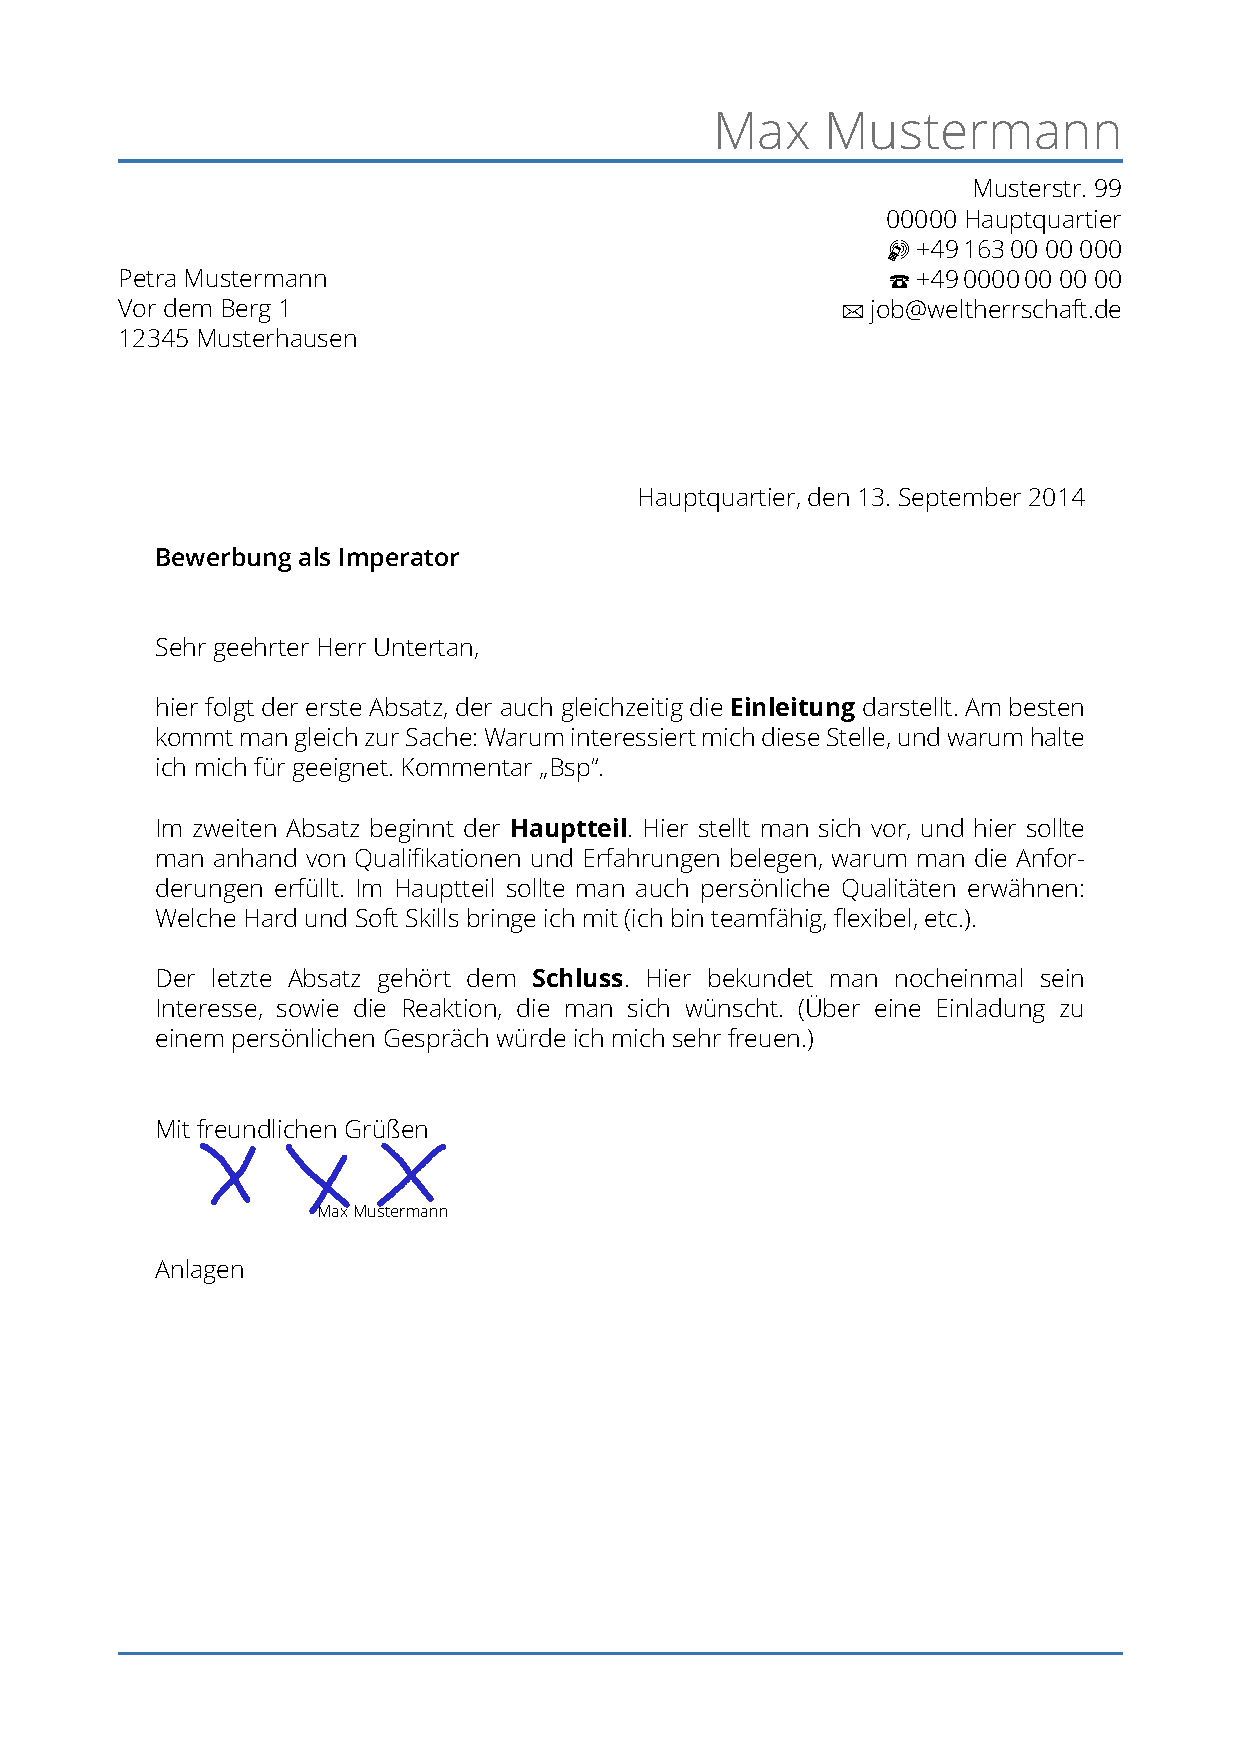
\includepdf[pages=-, addtotoc={1, pageRef, 0,Anschreiben,anschreiben}]{\anschreiben}
	\bookmark[page=\thepage,level=0]{Anschreiben}
	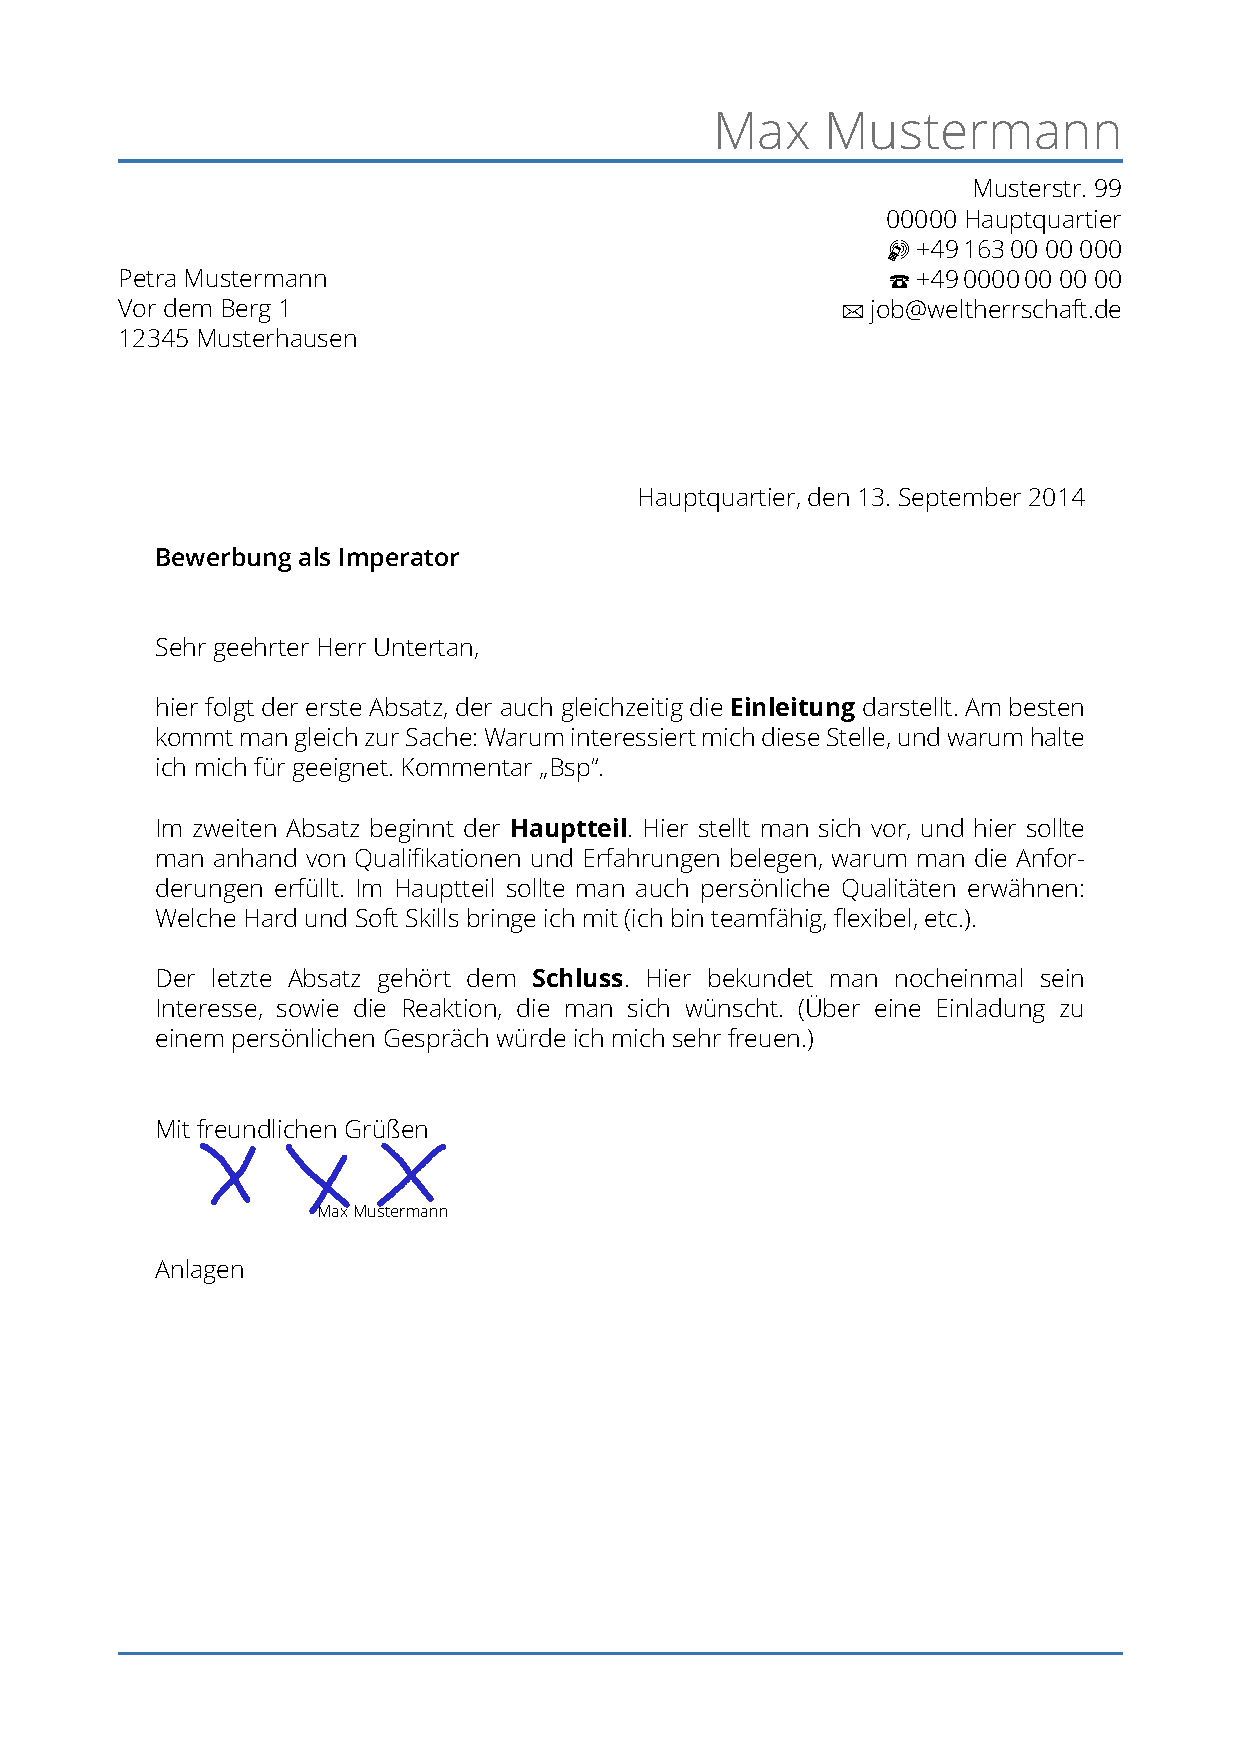
\includepdf[pages=-]{\anschreiben}
}{
	\Huge kein Anschreiben \newline
	\normalsize Im Pfad "\anschreiben" \hspace{1pt} konnte keine Datei gefunden werden. Bitte "\textbackslash buildir"\hspace{1pt}prüfen\newline
}
\IfFileExists{\lebenslauf}{
	%\includepdf[pages=-, addtotoc={1, pageRef, 0,Lebenslauf,lebenslauf}]{\lebenslauf}
	\bookmark[page=\thepage,level=0]{Lebenslauf}
	\includepdf[pages=-]{\lebenslauf}
}{
	\Huge kein CV\newline
	\normalsize Im Pfad "\lebenslauf" \hspace{1pt} konnte keine Datei gefunden werden. Bitte "\textbackslash buildir"\hspace{1pt}prüfen
}

% Weitere Anlagen
\newcommand* \pics {\priv Anhang/}

\bookmark[page=\thepage,level=0]{Abschlusszeugnisse}
\bookmark[page=\thepage,level=1]{Abitur: ...}
\includepdf[pages=-] {\pub ZeugnisBsp}%\anhang[1.7,\pics abi001.jpeg]
\anhang[4.0,\pub picture.jpg] %4x vergroessert
\bookmark[page=\thepage,level=1]{Diplom: ...}
\includepdf[pages=-] {\pub ZeugnisBsp}%\anhang[4.2,\pics studi1.jpeg]
\includepdf[pages=-] {\pub ZeugnisBsp}%\anhang[4.2,\pics studi1.jpeg]
\bookmark[page=\thepage,level=1]{Master: ...}
\includepdf[pages=-] {\pub ZeugnisBsp}%\anhangB(25,0,0,0)[3.7,\pics studi3.jpeg]
\includepdf[pages=-] {\pub ZeugnisBsp}%\anhang[4.2,\pics studi4.jpeg]

\bookmark[page=\thepage,level=0]{Arbeitszeugnisse}
\bookmark[page=\thepage,level=1]{Lalalala}
\includepdf[pages=-] {\pub ZeugnisBsp}
\bookmark[page=\thepage,level=1]{Fundação xxx}
\includepdf[pages=-] {\pub ZeugnisBsp}%\anhang[4.1,\pics xxx.jpeg]

\bookmark[page=\thepage,level=0]{Zertifikat}
\includepdf[pages=-] {\pub ZeugnisBsp}%\anhang[4.5,\pics xxx.jpeg]

\bookmark[page=\thepage,level=0]{Weitere Zeugnisse}
\bookmark[page=\thepage,level=1]{xxx - USA}
\includepdf[pages=-] {\pub ZeugnisBsp}%\anhang[0.72,\pics xxx.jpeg]
\bookmark[page=\thepage,level=1]{xxxx - Brasilien}
\includepdf[pages=-] {\pub ZeugnisBsp}%\anhang[9,\pics xx.jpeg]
\end{document}